\section{Simulation Analysis}
\label{sec:simulation}

\subsection{Operating Point Analysis}

Table~\ref{tab:op} shows the simulated operating point results for the circuit
under analysis. Compared to the theoretical analysis results, one notices the
following differences: describe and explain the differences.

\begin{table}[h]
  \centering
  \begin{tabular}{|l|r|}
    \hline    
    {\bf Name} & {\bf Value [A or V]} \\ \hline
    n2 (V) & 5.070727e+00\\ \hline
n3 (V) & 4.825468e+00\\ \hline
n4 (V) & 4.304579e+00\\ \hline
n5 (V) & 4.860091e+00\\ \hline
n6 (V) & 8.720760e+00\\ \hline
n7 (V) & -2.93990e+00\\ \hline
n8 (V) & -1.95020e+00\\ \hline
Vc (V) & 7.799989e+00\\ \hline
r1 (A) & -2.40330e-04\\ \hline
r2 (A) & -2.51475e-04\\ \hline
r3 (A) & -1.11453e-05\\ \hline
r4 (A) & -1.20919e-03\\ \hline
r5 (A) & -1.25166e-03\\ \hline
r6 (A) & 9.688613e-04\\ \hline
r7 (A) & 9.688613e-04\\ \hline
Ib (A) & -2.51475e-04\\ \hline

  \end{tabular}
  \caption{Operating point. A variable preceded by @ is of type {\em current}
    and expressed in Ampere; other variables are of type {\it voltage} and expressed in
    Volt.}
  \label{tab:op}
\end{table}

\lipsum[1-1]

\subsection{Transient Analysis}

%Figure~\ref{fig:trans} shows the simulated transient analysis results for the
circuit under analysis. Compared to the theoretical analysis results, one
notices the following differences: describe and explain the differences.

%\begin{figure}[h] \centering
%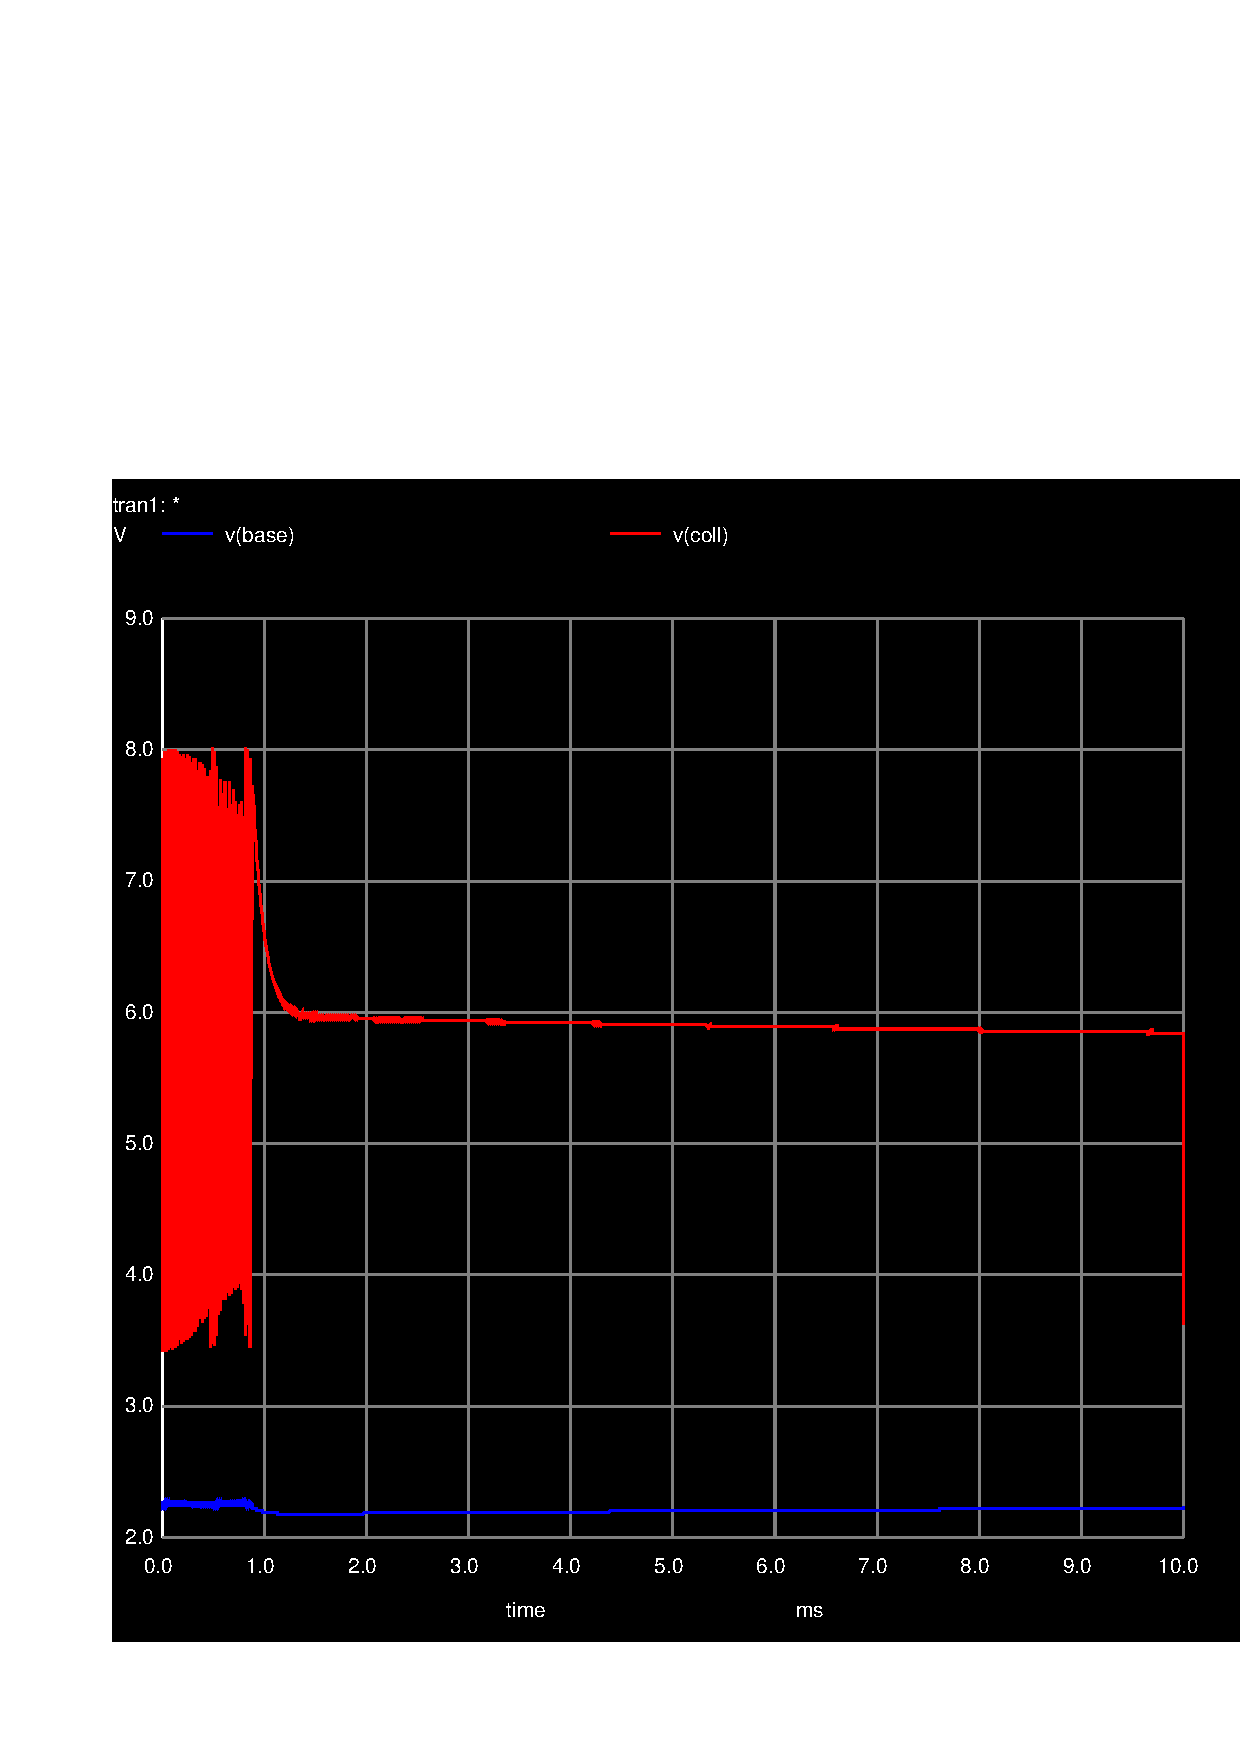
\includegraphics[width=0.6\linewidth]{trans.pdf}
%\caption{Transient output voltage}
%\label{fig:trans}
%\end{figure}

\lipsum[1-1]



\subsection{Frequency Analysis}

\subsubsection{Magnitude Response}

%Figure~\ref{fig:acm} shows the magnitude of the frequency response for the
circuit under analysis. Compared to the theoretical analysis results, one
notices the following differences: describe and explain the differences.

%\begin{figure}[h] \centering
%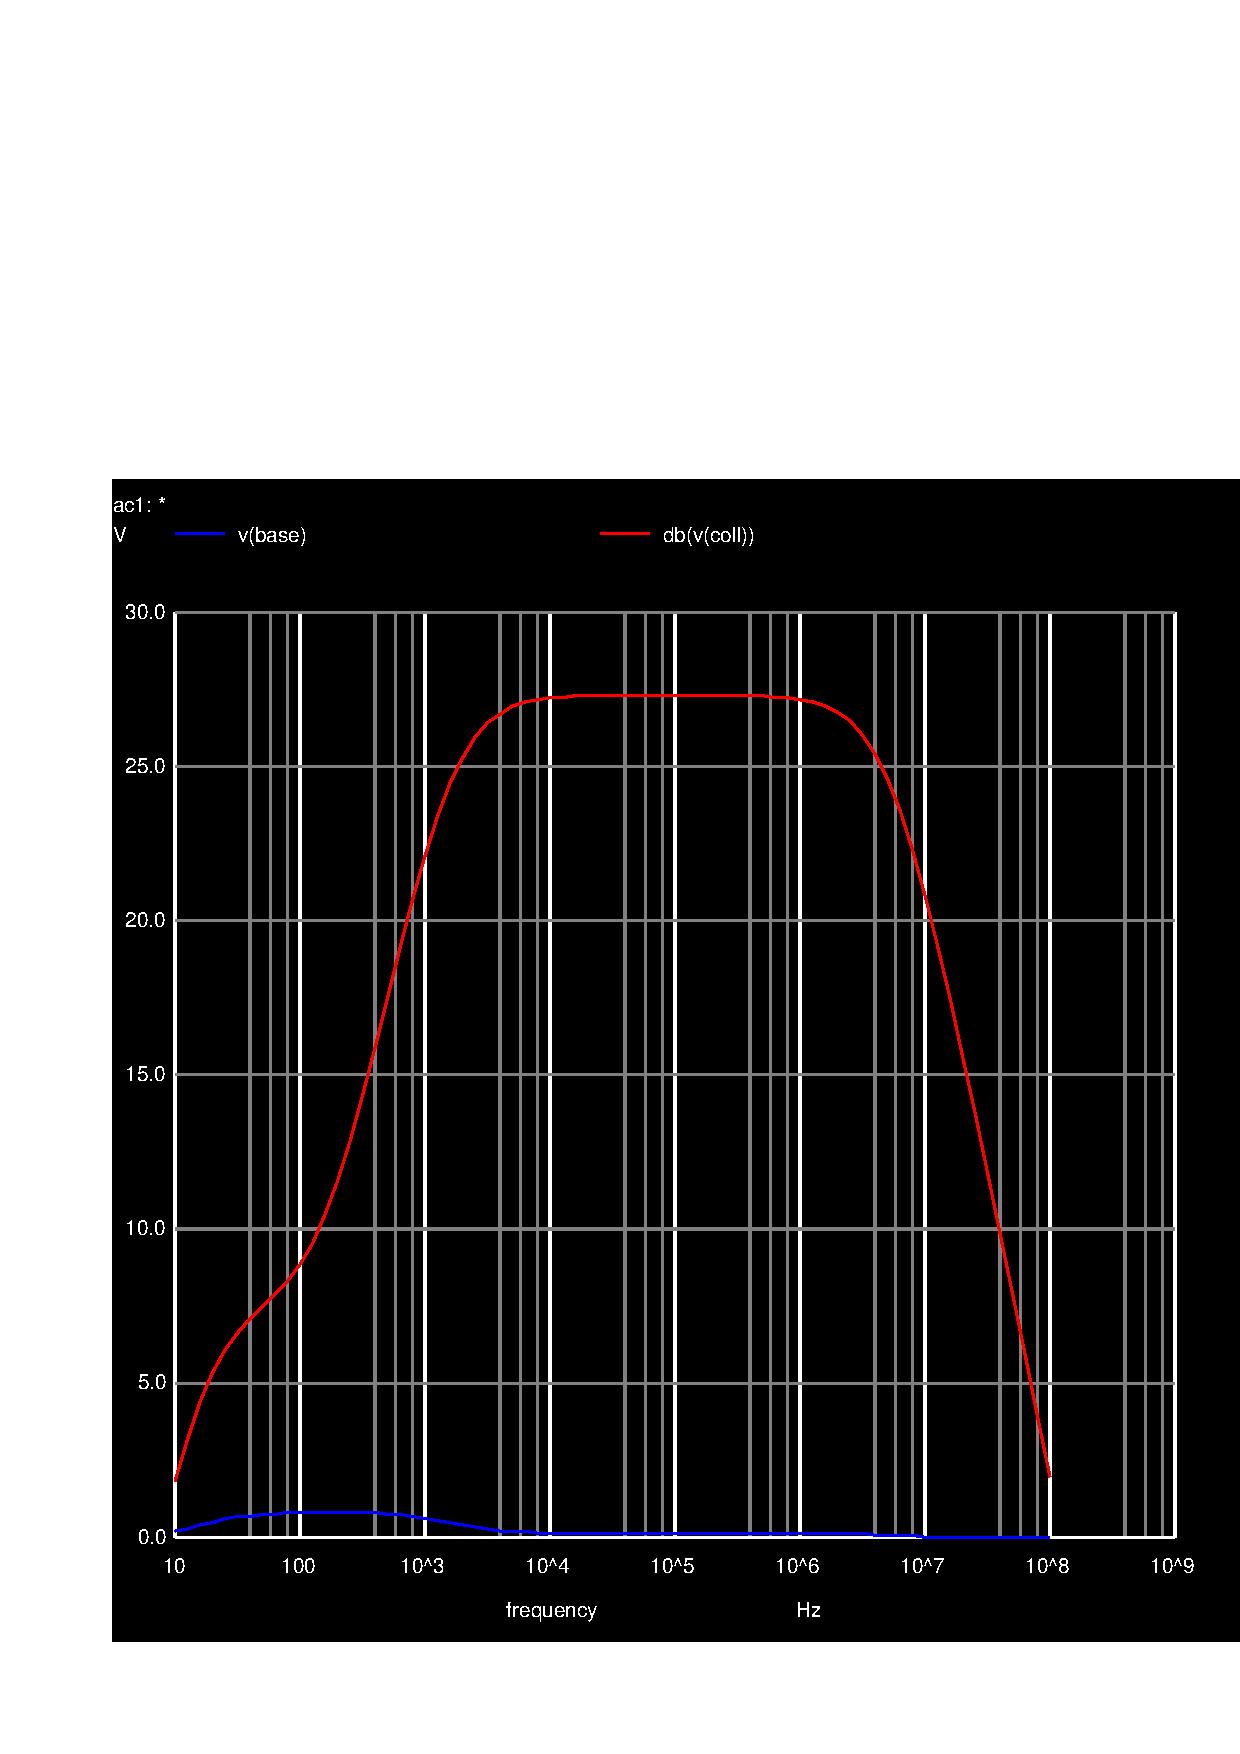
\includegraphics[width=0.6\linewidth]{acm.pdf}
%\caption{Magnitude response}
%\label{fig:acm}
%\end{figure}

\lipsum[1-1]

\subsubsection{Phase Response}

%Figure~\ref{fig:acp} shows the magnitude of the frequency response for the
circuit under analysis. Compared to the theoretical analysis results, one
notices the following differences: describe and explain the differences.

%\begin{figure}[h] \centering
%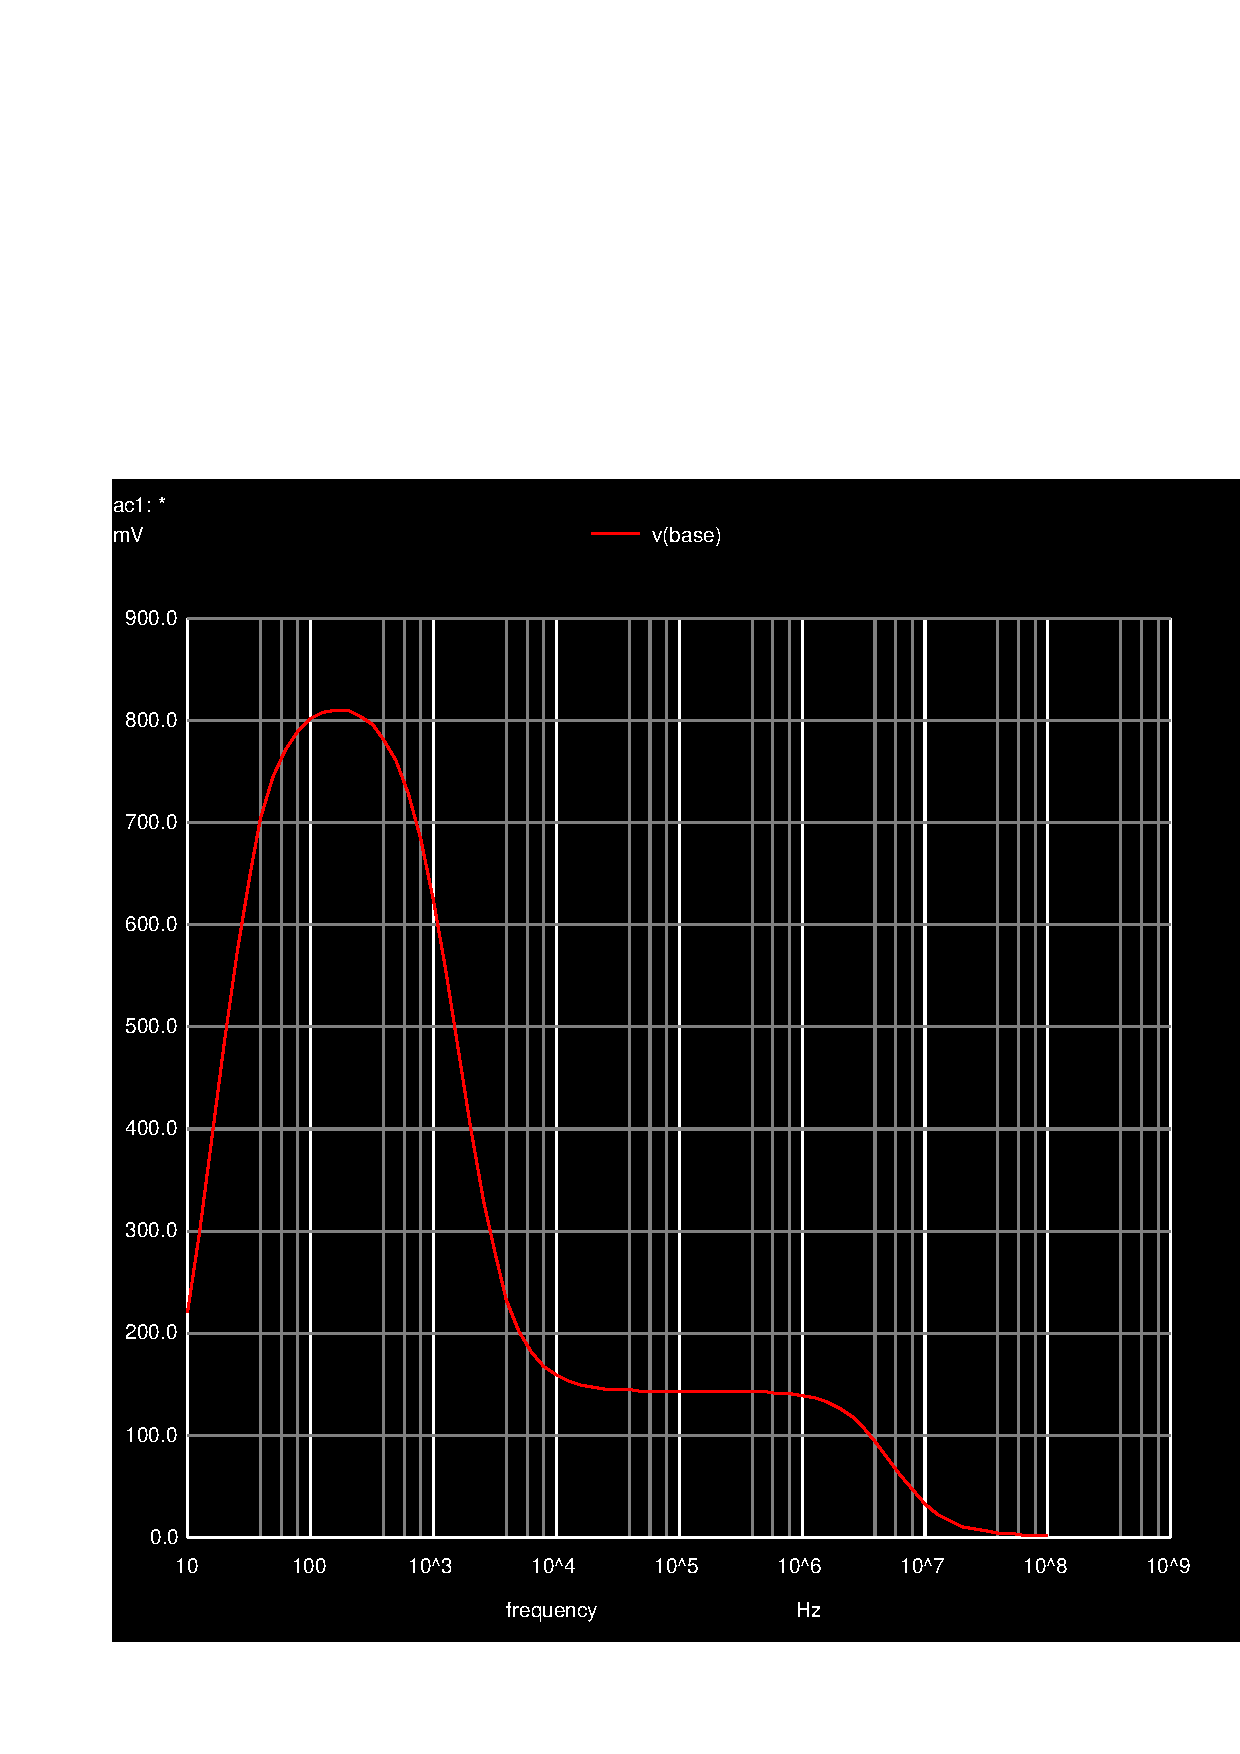
\includegraphics[width=0.6\linewidth]{acp.pdf}
%\caption{Phase response}
%\label{fig:acp}
%\end{figure}

\lipsum[1-1]

\subsubsection{Input Impedance}

%Figure~\ref{fig:zim} shows the magnitude of the frequency response for the
circuit under analysis. Compared to the theoretical analysis results, one
notices the following differences: describe and explain the differences.

%\begin{figure}[h] \centering
%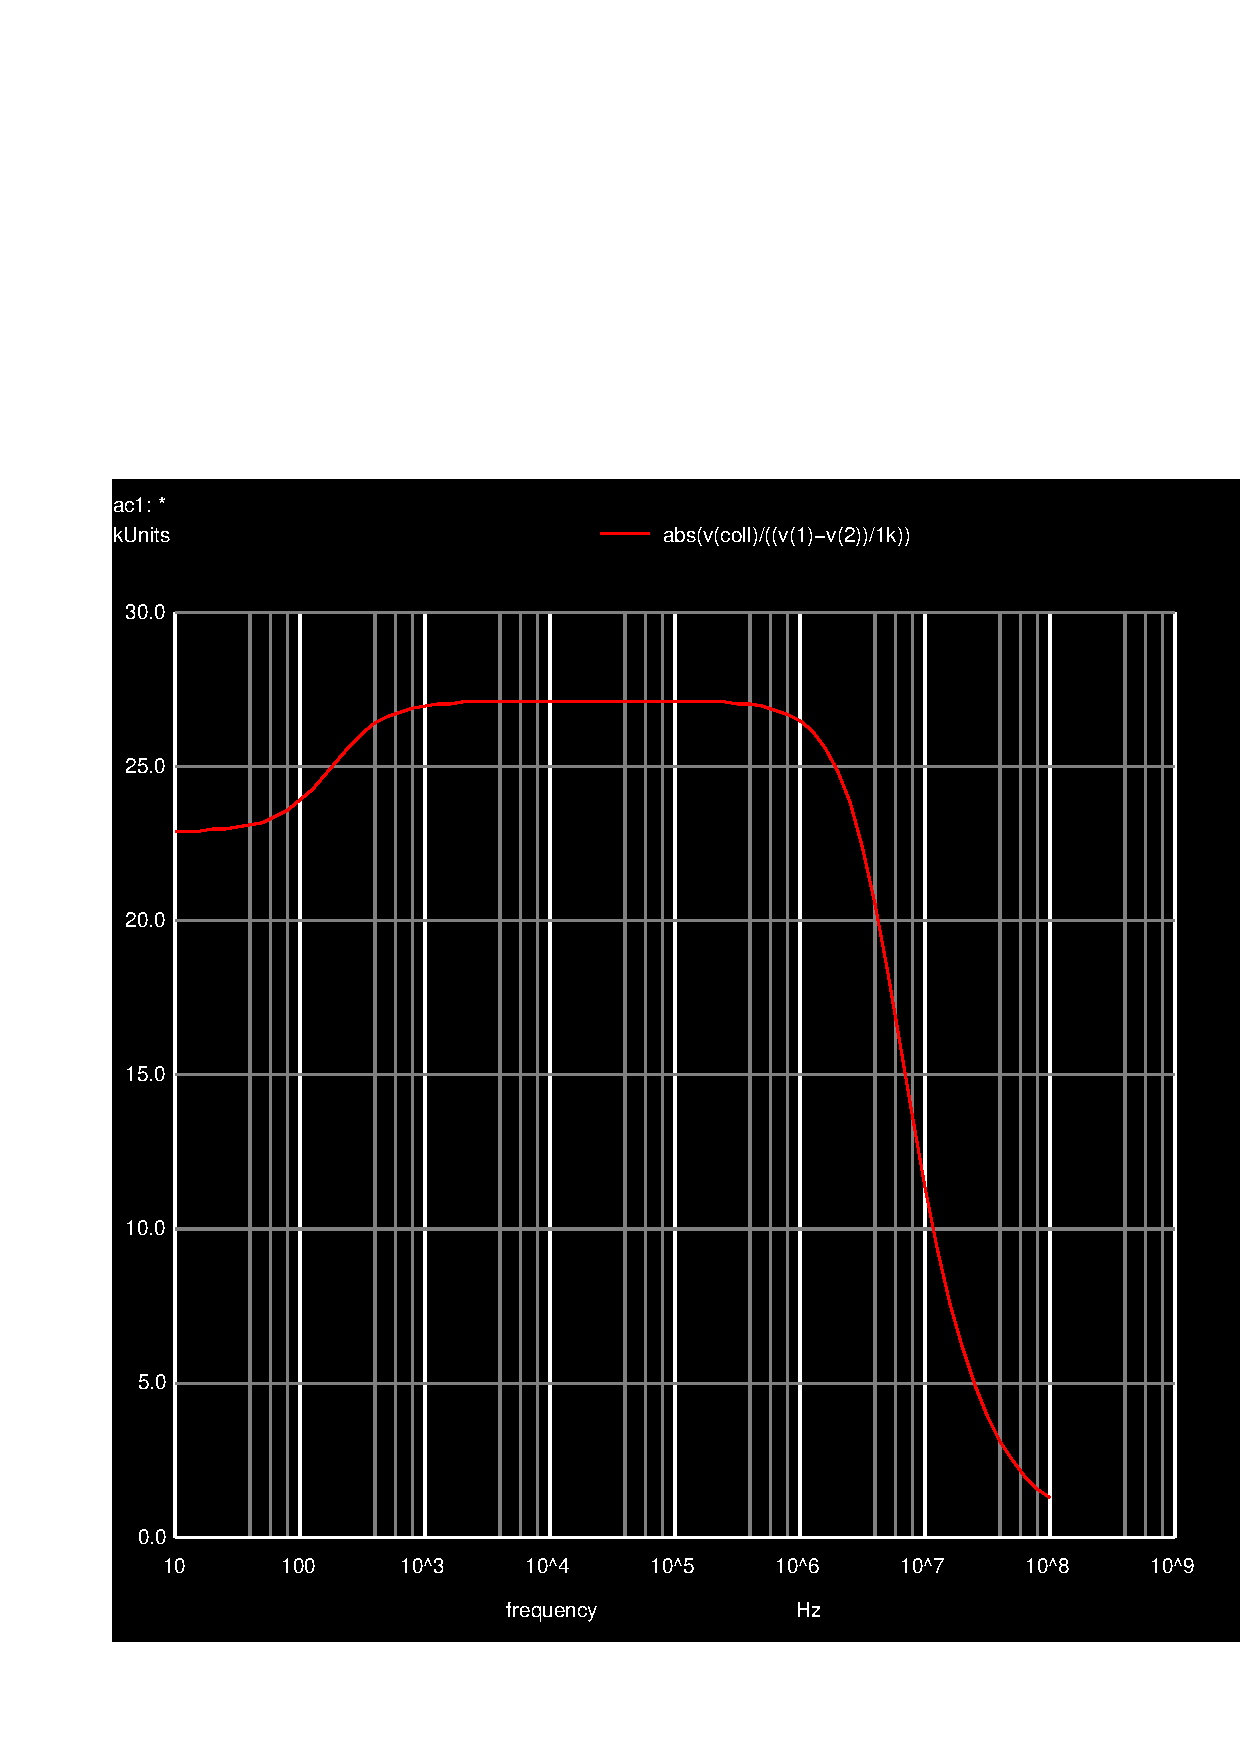
\includegraphics[width=0.6\linewidth]{zim.pdf}
%\caption{Input impedance}
%\label{fig:zim}
%\end{figure}

\lipsum[1-1]



